
\subsection{Data science process}
There are many different lifecycle models to describe phases in a data science project. This section will give a quick overview of some important ones.


We'll start with \textbf{CRISP-DM}\sidenote{CRISP-DM} which stands for "Cross-industry standard process for data mining". It was developed in the late 1990s by different involved companies \textcolor{gray}{\footnotesize(SPSS, Teradata, Daimler AG, NCR Corporation, Ohra)}. The process consists of multiple steps playing together as visualized in \ref{fig:1_crisp_dm}

\begin{figure}[H]
  \centering
  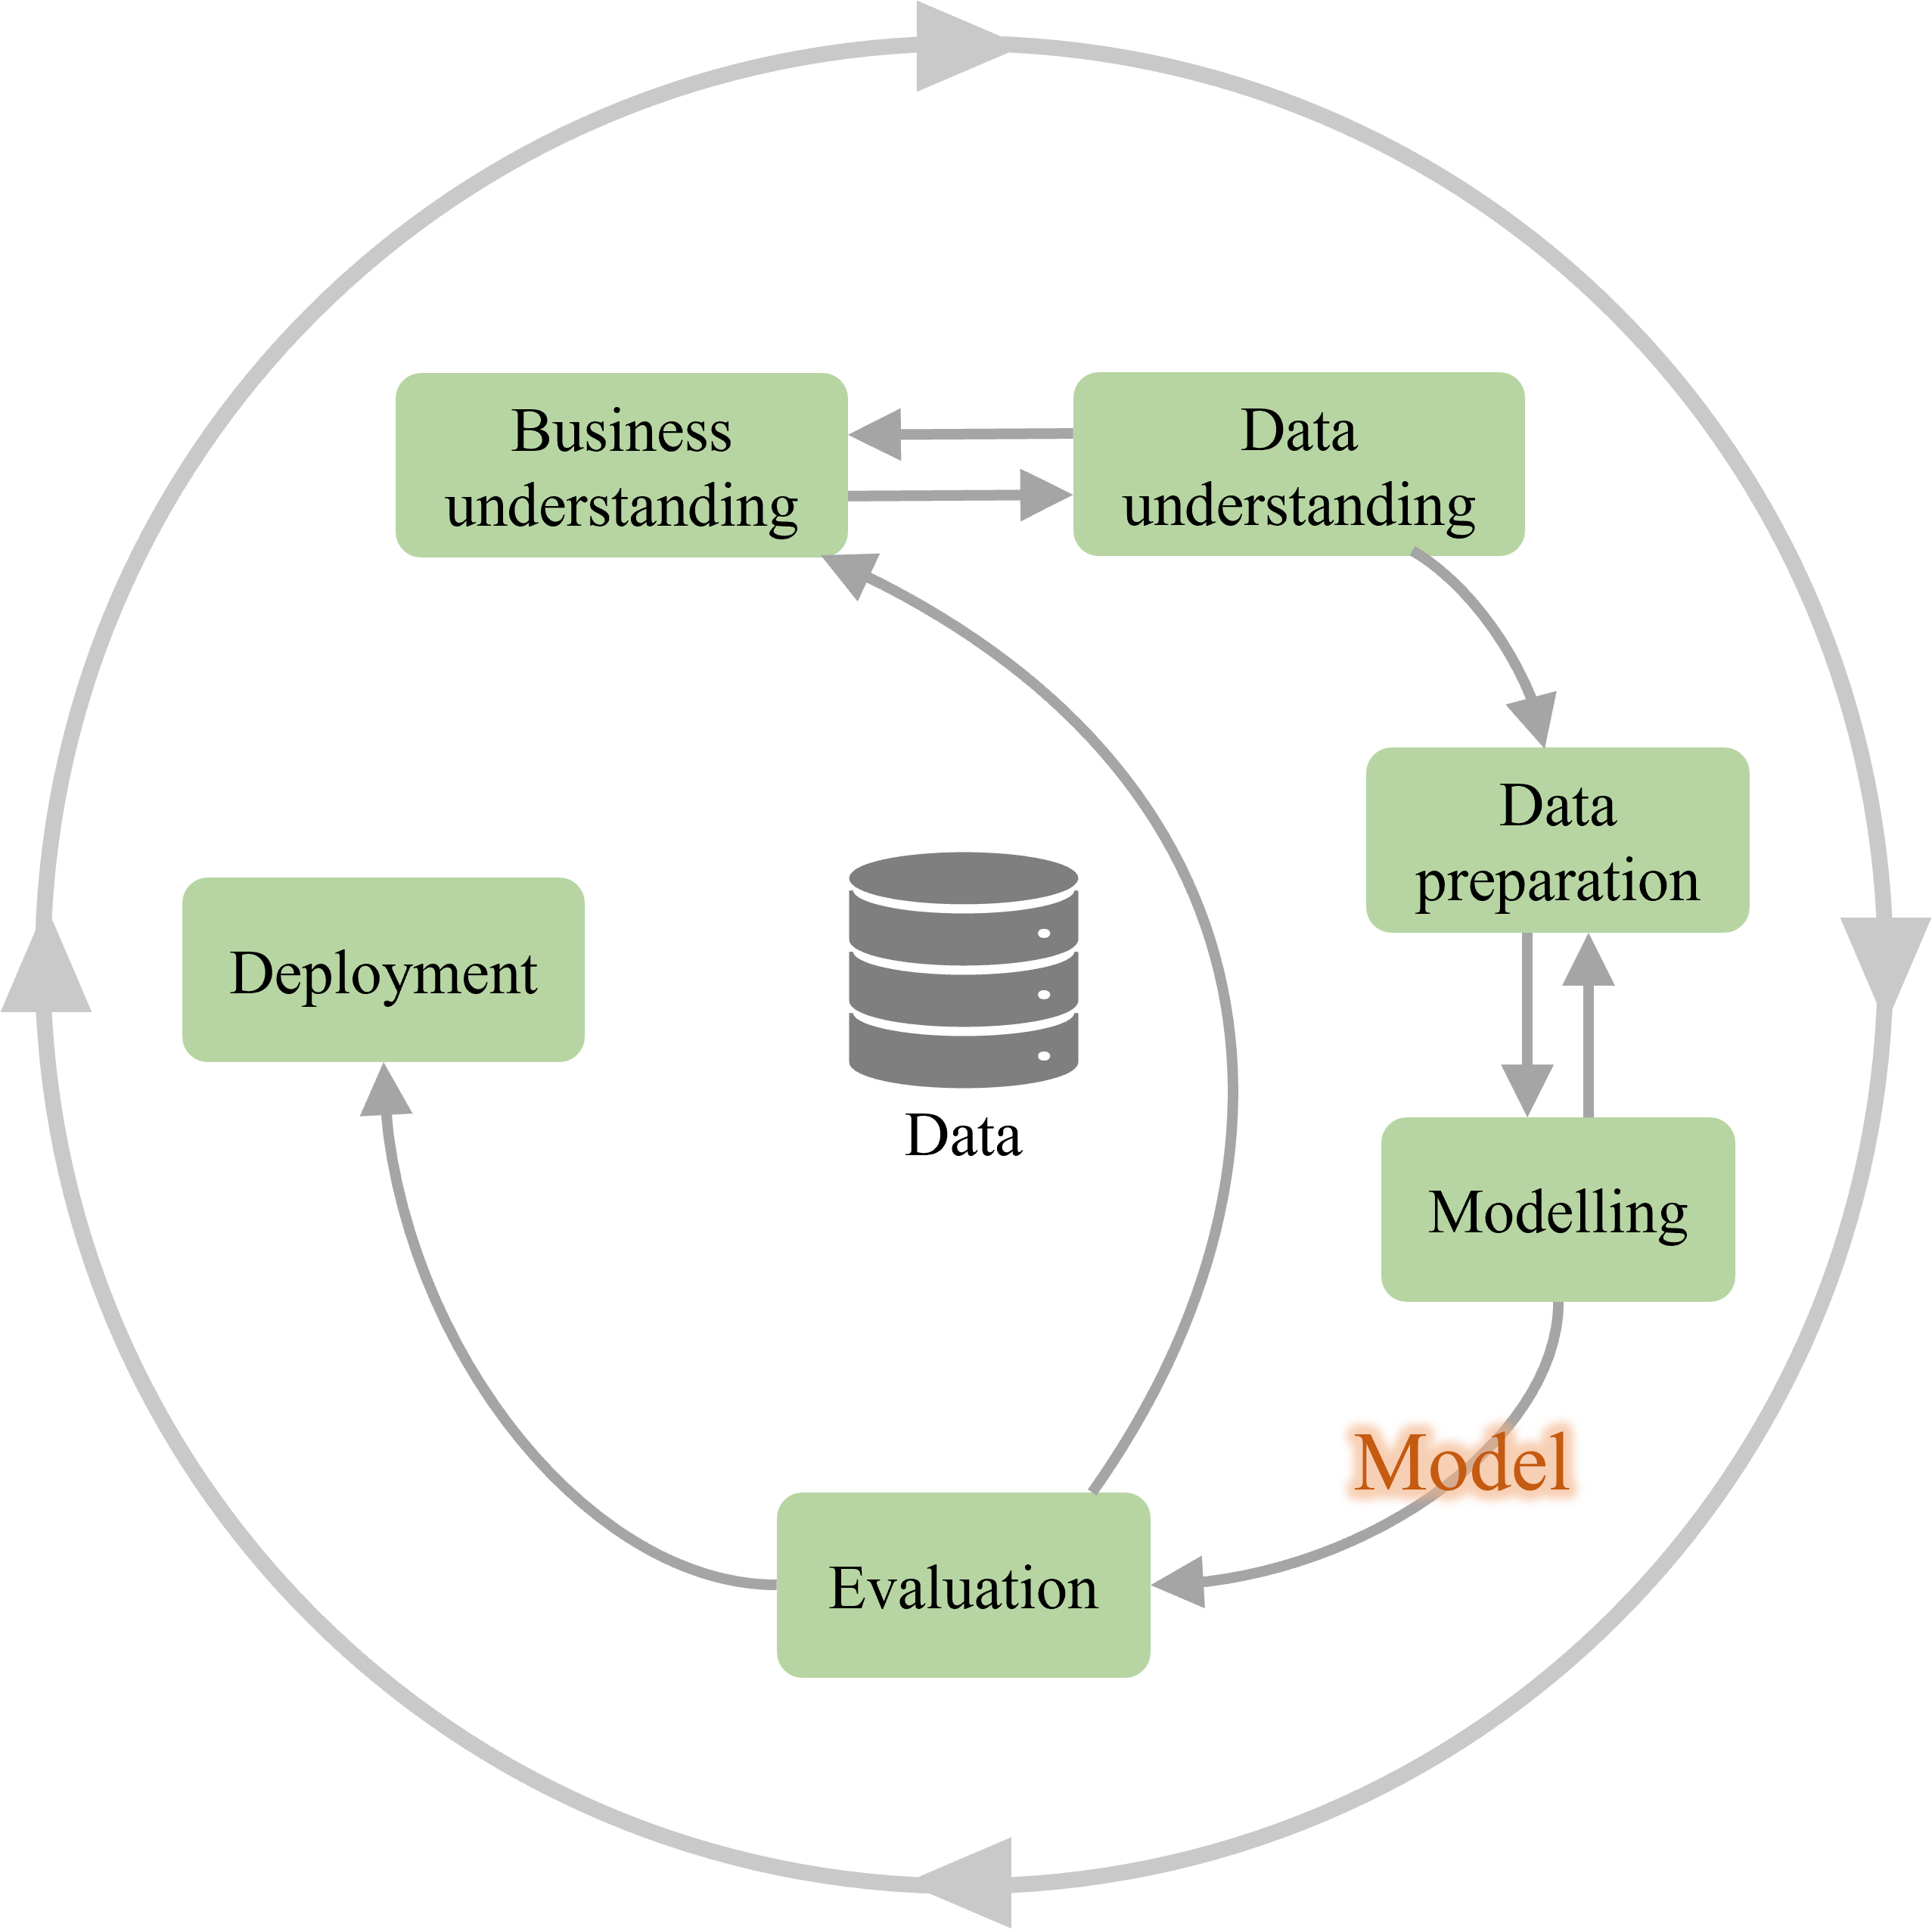
\includegraphics[width=0.7\textwidth]{assets/basics/crisp-dm.png}
  \caption{CRISP-DM process}
  \label{fig:1_crisp_dm}
\end{figure}

\begin{longtable}{>{\color{black}}p{0.4\linewidth} >{\color{gray}\footnotesize}p{0.6\linewidth}}
  \multicolumn{2}{l}{\textbf{Business understanding}} \\
  $\quad$Determine business objective & Background, business objective, business success criteria \\
  $\quad$Situation assessment & Inventory of resources, requirements, assumptions, constraints, risks, contingencies, terminology, costs, benefits \\
  $\quad$Determine data mining goal & Data mining goals, data mining success criteria \\
  $\quad$Produce project plan & Project plan, initial assessment of tools and techniques \\[5pt]
  
  \multicolumn{2}{l}{\textbf{Data understanding}} \\
  $\quad$Collect initial data & Initial data collection report \\
  $\quad$Describe and explore data & Data description, exploration report \\
  $\quad$Verify data quality & Data quality report \\[5pt]
  
  \multicolumn{2}{l}{\textbf{Data preparation} (Starting point: data set \textcolor{gray}{\footnotesize data set with description})} \\
  $\quad$Select data & Rationale for inclusion and exclusion \\
  $\quad$Clean data & Data cleaning report \\
  $\quad$Construct data & Derived attributes, generated records \\
  $\quad$Integrate and format data & Merged/reformatted data \\[5pt]
  
  \multicolumn{2}{l}{\textbf{Modeling}\footnote{The term "modeling" can be misleading. Meant is the selection and assumptions by a human, or automated learning by a tool or algorithm}} \\
  $\quad$Select modeling technique & Modeling technique, modeling assumptions \\
  $\quad$Generate test design & Test design \\
  $\quad$Build model & Parameter settings, models, model description \\
  $\quad$Assess model & Model assessment, revised parameter settings \\[5pt]
  
  \multicolumn{2}{l}{\textbf{Evaluation}} \\
  $\quad$Evaluate results & Assessment of data mining results w.r.t. business success criteria, approved models \\
  $\quad$Review process & Review of process \\
  $\quad$Determine next steps & List of possible actions settings \\[5pt]
  
  \multicolumn{2}{l}{\textbf{Deployment}} \\
  $\quad$Plan deployment & Deployment plan \\
  $\quad$Plan monitoring, maintenance & Monitoring and maintenance plan \\
  $\quad$Produce final report & Final report and final presentation \\
  $\quad$Review project & Experience documentation
  
\end{longtable}

Next, we have the \textbf{KDD}\sidenote{KDD} (Knowledge Discovery in Databases) process as shown in \ref{fig:1_kdd}. Another process model also developed by SAS institute is called \textbf{SEMMA}\sidenote{SEMMA} consisting of the phases Sample, Explore, Modify, Model, and Assess.

\begin{figure}[H]
  \centering
  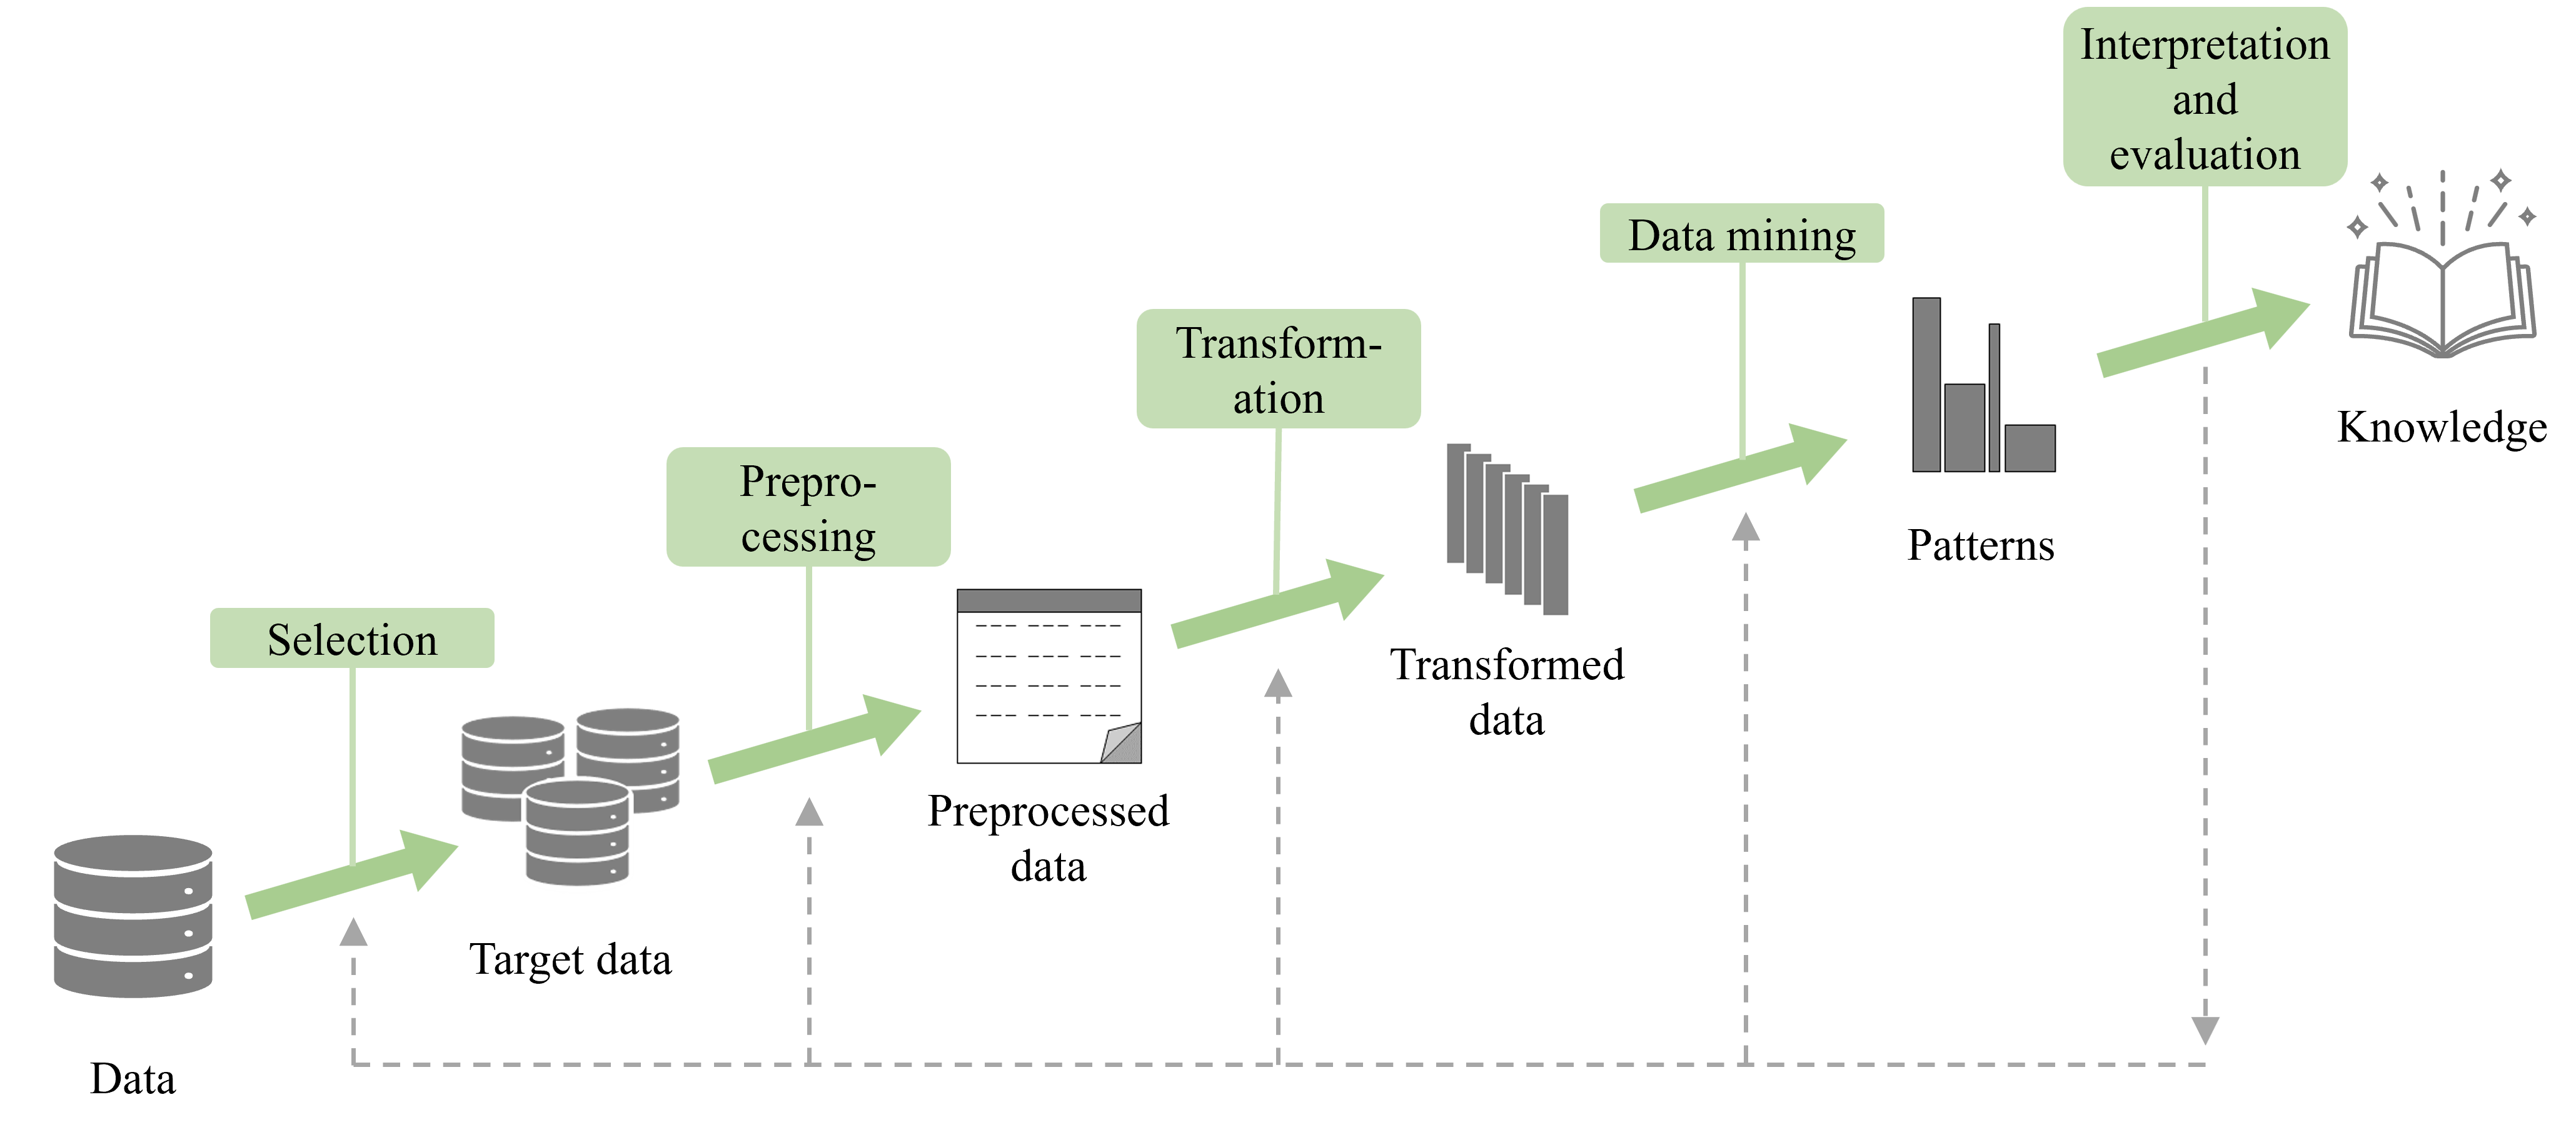
\includegraphics[width=\textwidth]{assets/basics/kdd.png}
  \caption{KDD process}
  \label{fig:1_kdd}
\end{figure}


The next process model is specifically developed for \textbf{L* lifecycle model}\sidenote{L* lifecycle model} with multiple stages as shown in \ref{fig:1_l_star}. 

\begin{figure}[H]
  \centering
  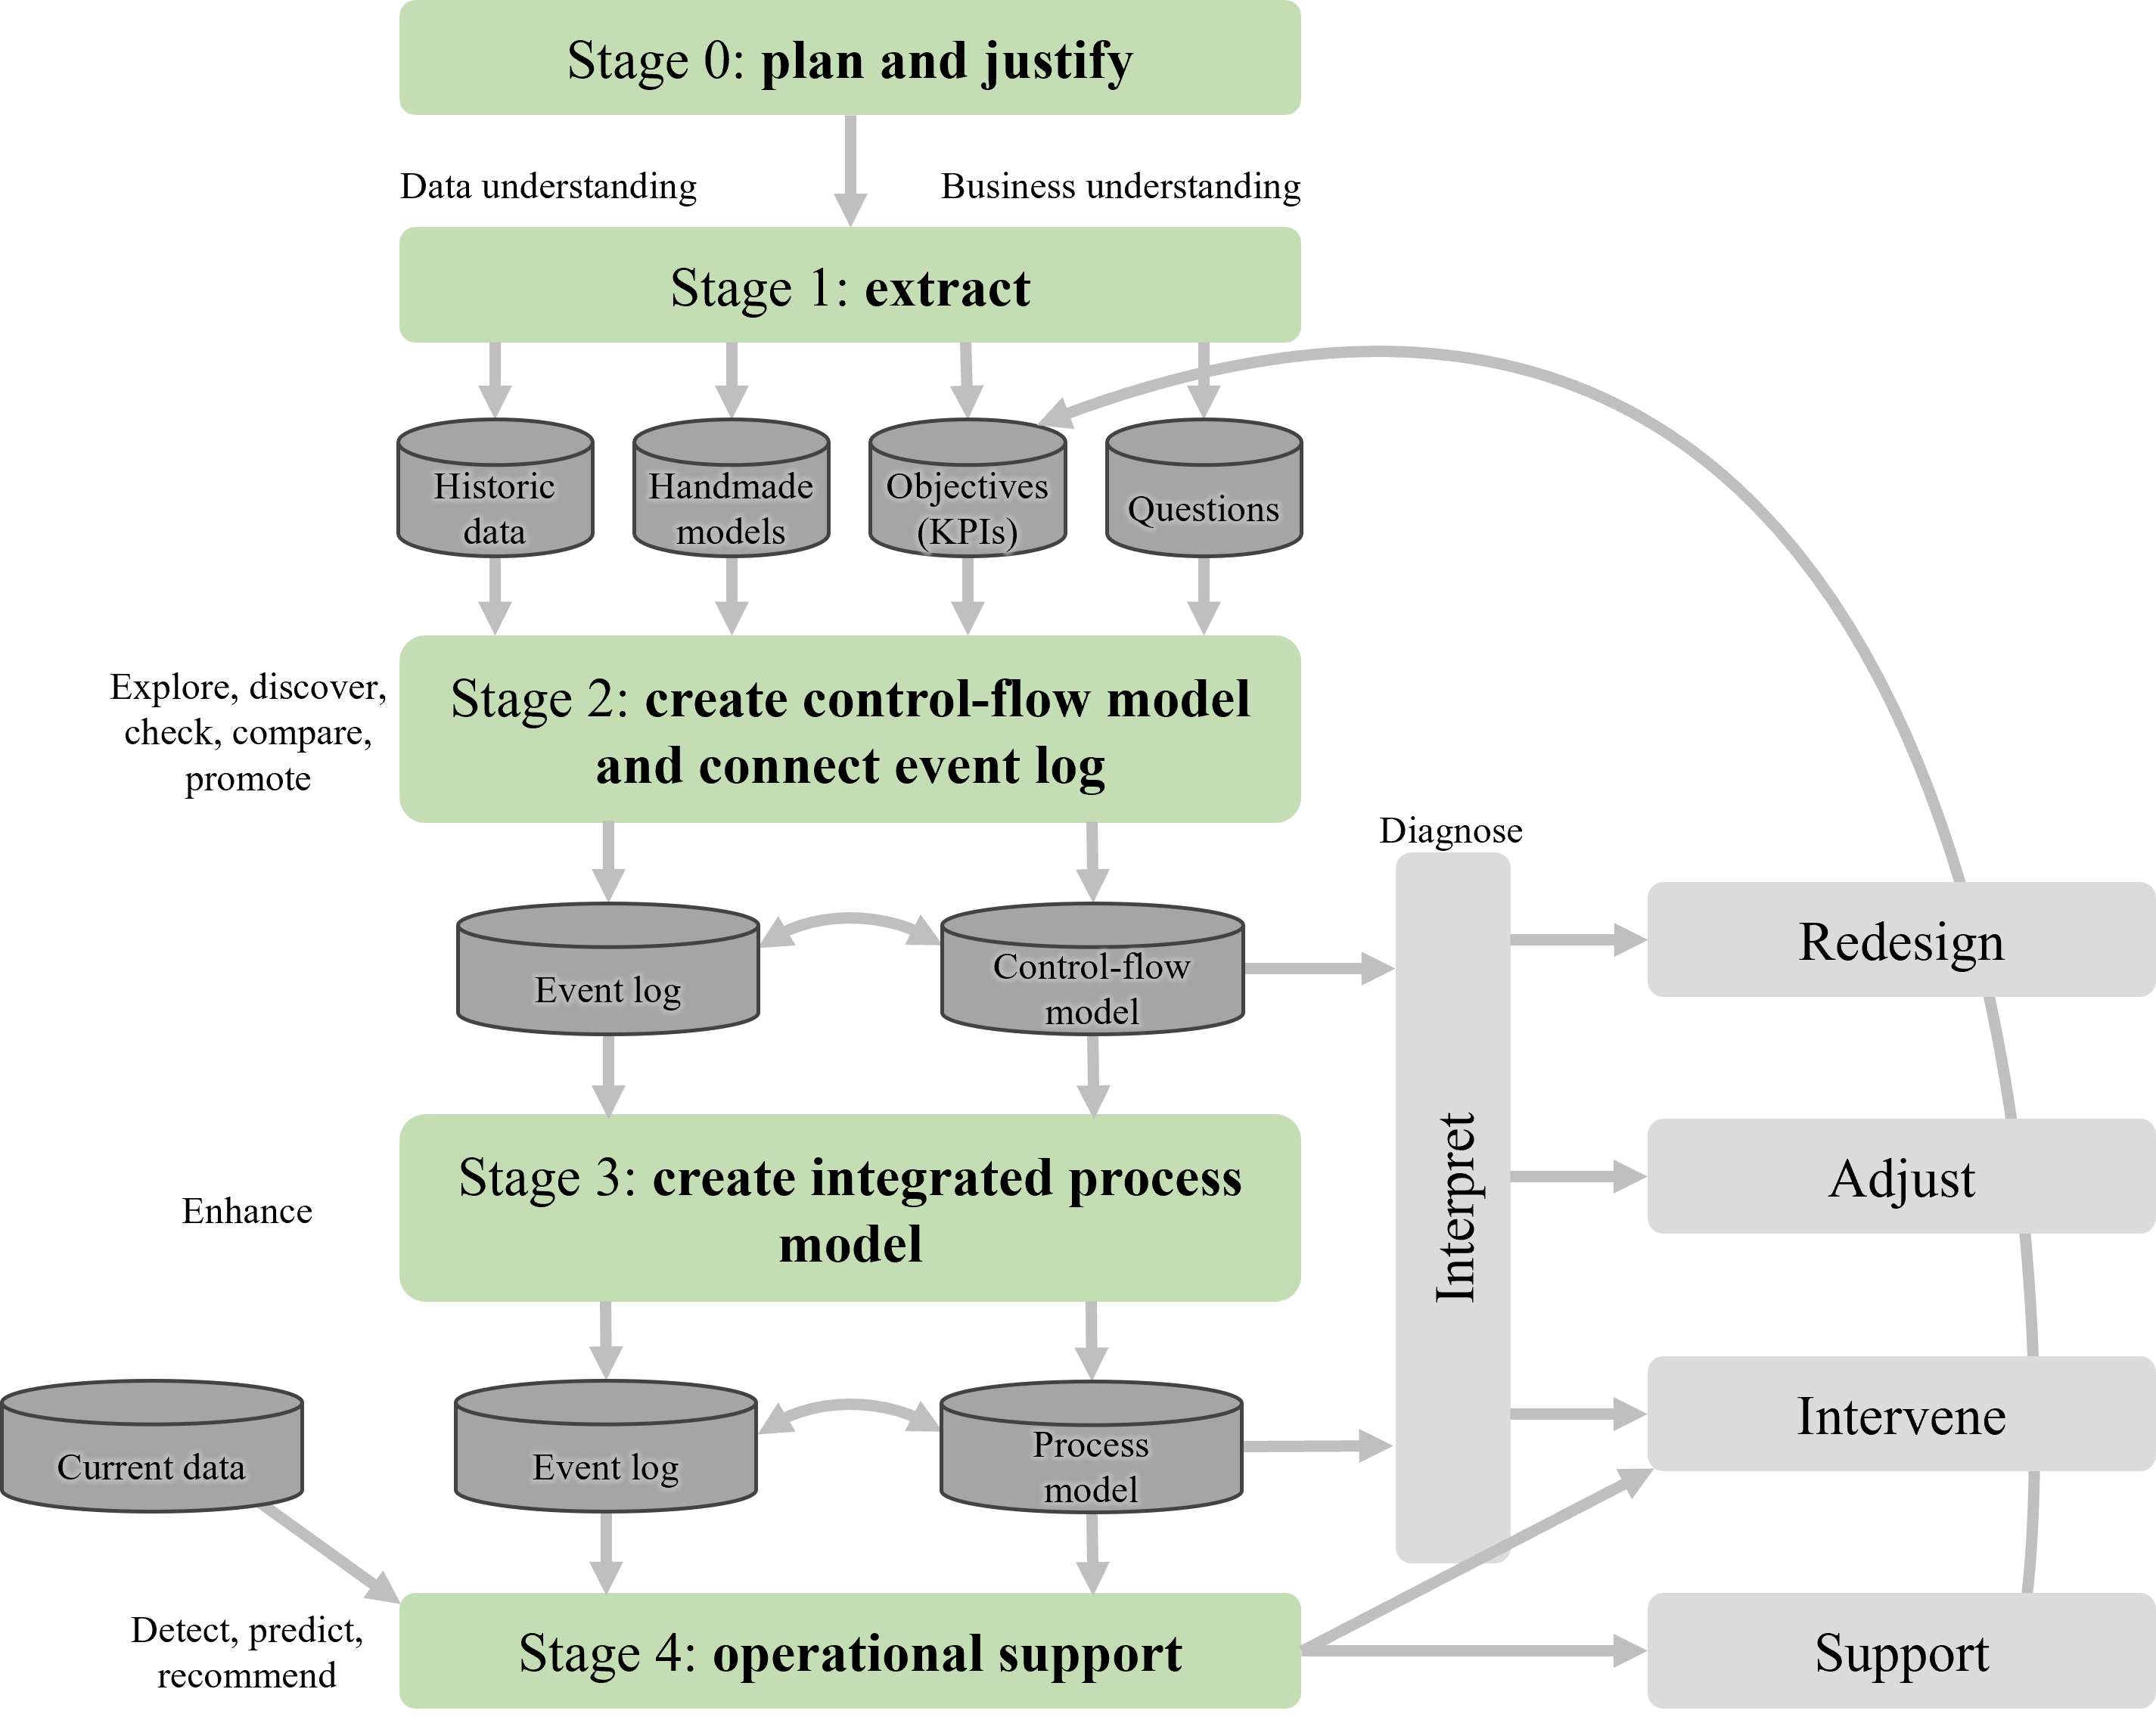
\includegraphics[width=0.75\textwidth]{assets/basics/l_star.png}
  \caption{L* lifecycle model}
  \label{fig:1_l_star}
\end{figure}


Furthermore, we have two methodologies the process model can be related to. Important to implement and solidify are improvements in both.
\begin{itemize}
  \item \textbf{PDCA}\sidenote{PDCA} stands for Plan-Do-Check-Act and is a never-ending cycle with exactly these steps. 
  \item The other one \textbf{DMAIC}\sidenote{DMAIC} stands for Define-Measure-Analyze-Improve-Control, with the following subtasks:
  \begin{itemize}
    \item {\color{gray}\footnotesize Define: launch team, establish charter, plan project, gather VOC/VOB, plan for change}
    \item {\color{gray}\footnotesize Measure: document process, collect baseline data, narrow project focus}
    \item {\color{gray}\footnotesize Analyze: analyze data, identify root causes, identify and remove waste}
    \item {\color{gray}\footnotesize Improve: generate, evaluate, and optimize solutions, pilot, plan and implement}
    \item {\color{gray}\footnotesize Control: control the process, validate project benefits}
  \end{itemize}
\end{itemize}


Finally, we have two processes with the same components, but different ordering of the steps as can be seen in \ref{fig:1_etl_and_elt}. The short terms for the processes are \textbf{ETL}\sidenote{ETL} (extract, transform, load) and \textbf{ELT}\sidenote{ELT} (extract, load, transform).

\begin{figure}[H]
  \centering

  \subcaptionbox{ETL with data warehouse}{
    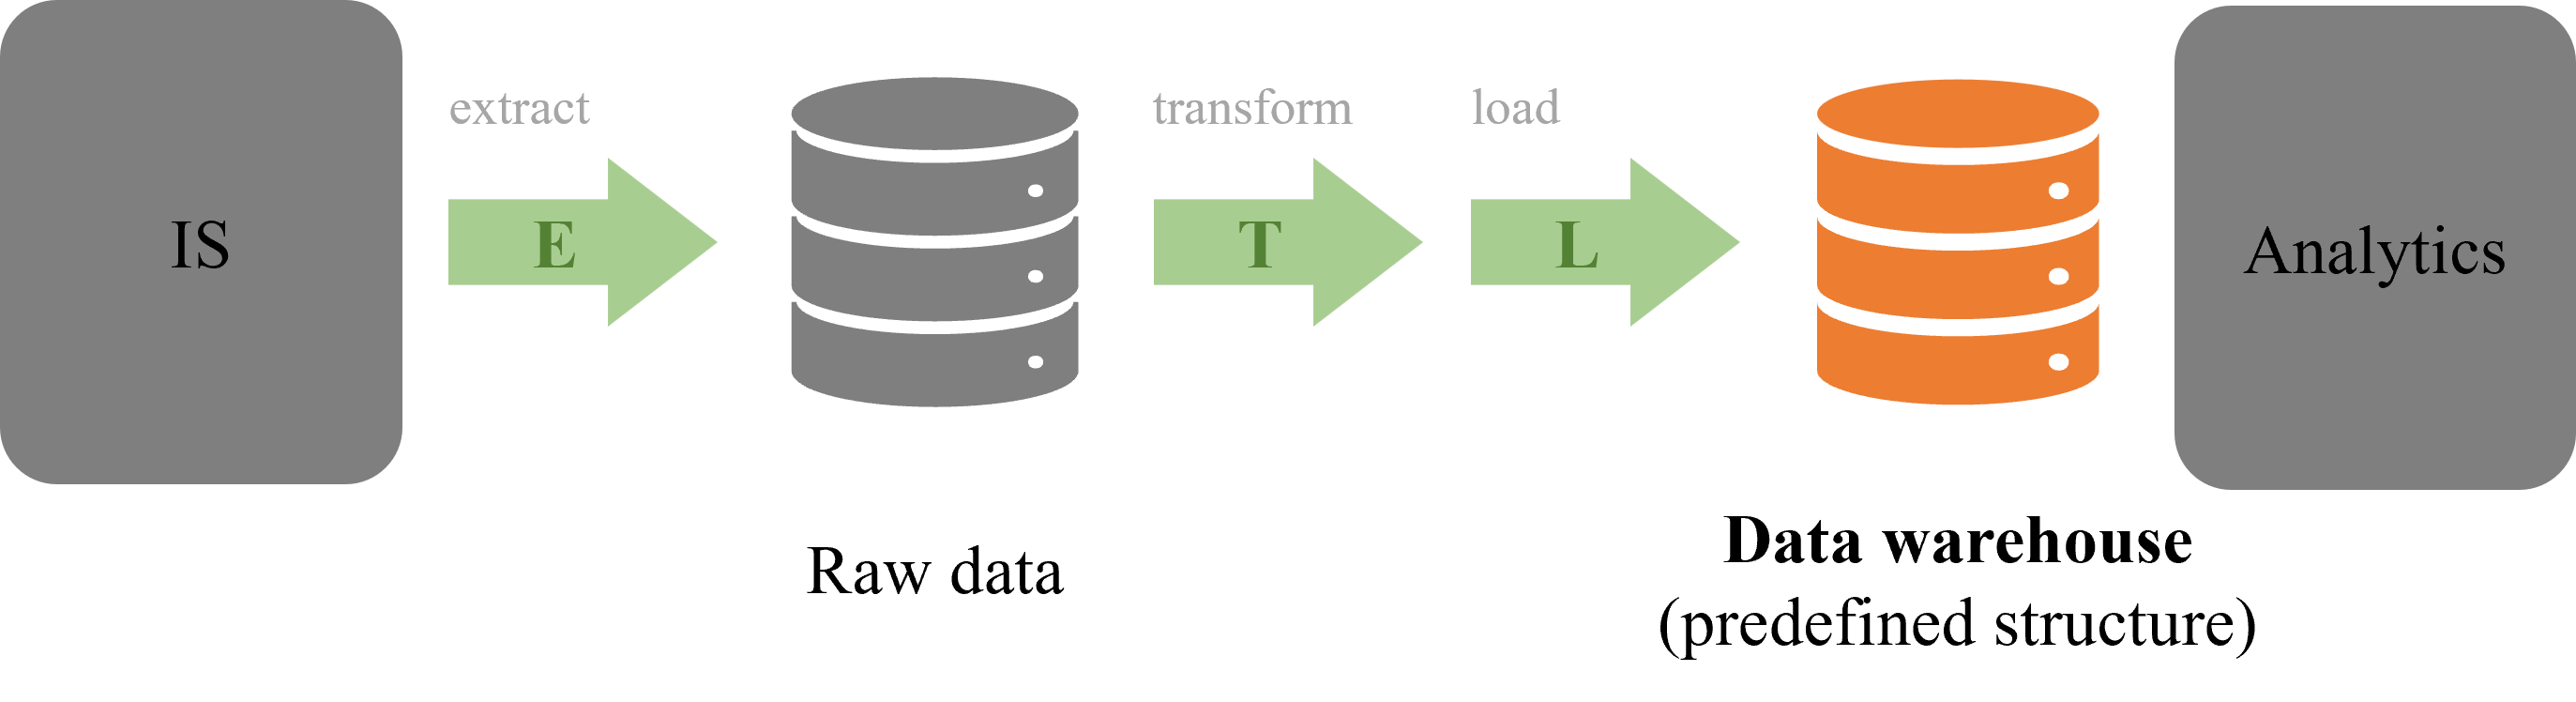
\includegraphics[width=0.5\textwidth]{assets/basics/etl.png}
  }
  \\\vspace*{0.5cm}
  \subcaptionbox{ELT with data lake}{
    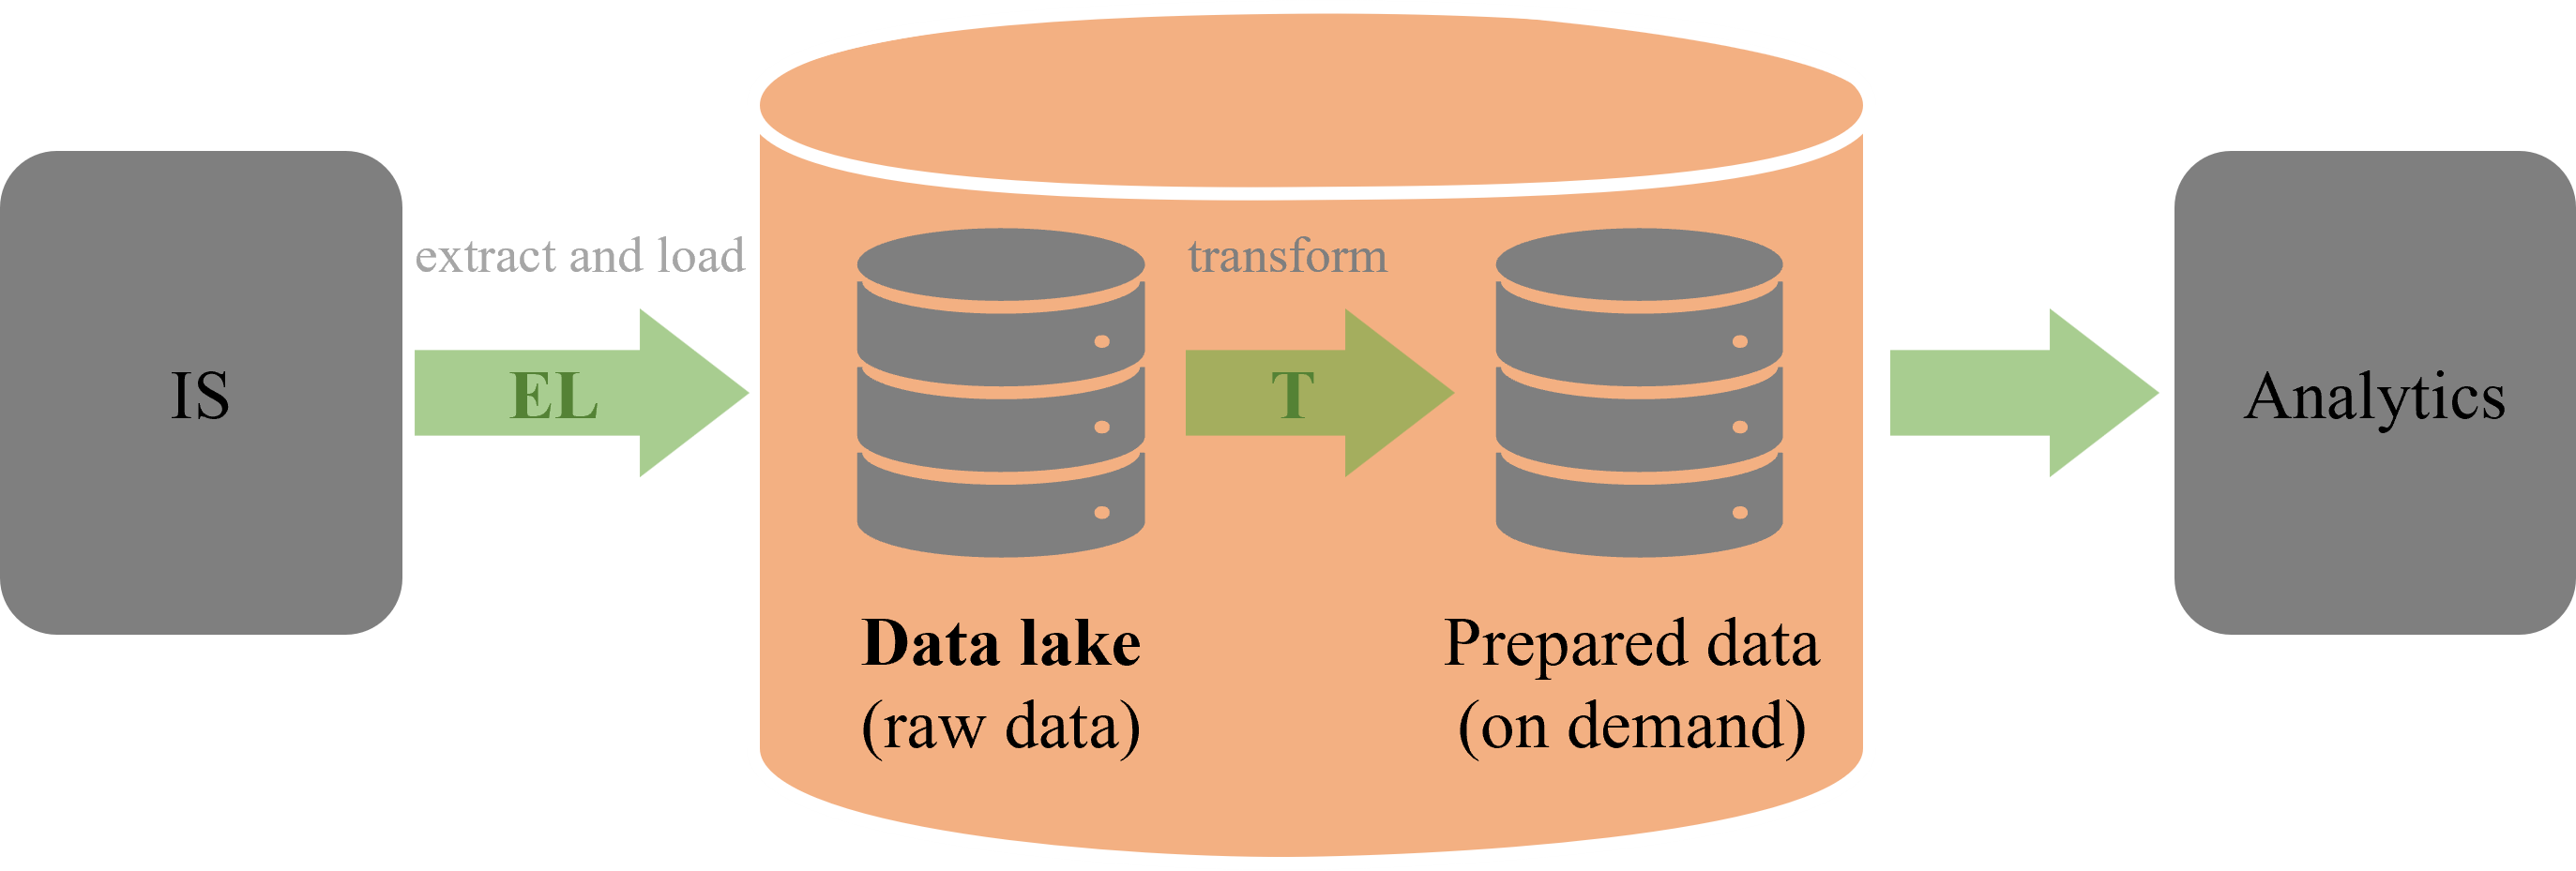
\includegraphics[width=0.5\textwidth]{assets/basics/elt.png}
  }

  \caption{Processes with extraction, transform, and load steps}
  \label{fig:1_etl_and_elt}
\end{figure}

\subsubsection*{80/20 rule}
As a final note on which steps are usually the most time-expensive: there is a so-called "80/20 rule" stating:
\begin{itemize}
  \item 80\% of a data scientist's time is spent on finding, cleaning, preprocessing, and organizing data. This leaves only 20\% to actually perform an analysis.
  \item On the other hand, we have 20\% effort determining 80\% of the final result.
\end{itemize}

\begin{figure}[H]
  \centering
  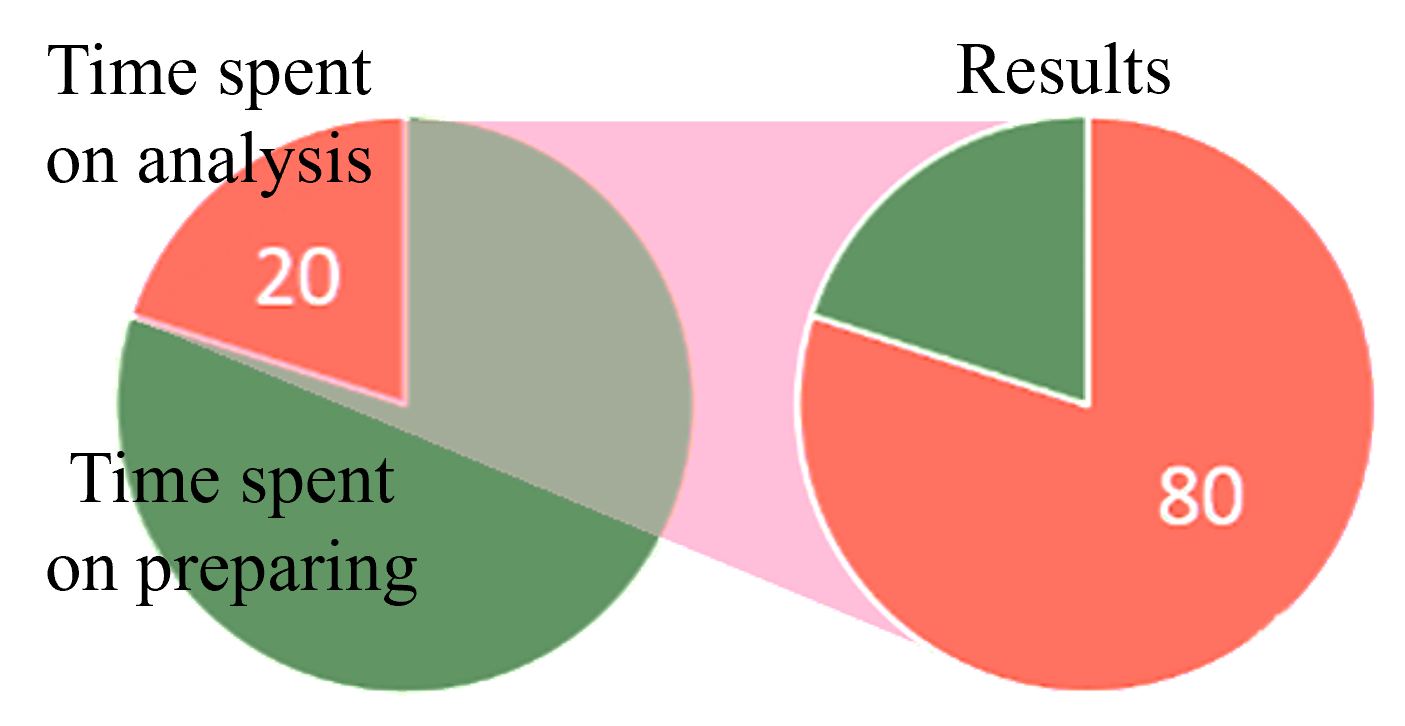
\includegraphics[width=0.4\textwidth]{assets/basics/80_20.png}
  \caption{80-20 rule}
  \label{fig:1_80_20}
\end{figure}